\subsection{Urban Micro Scenario}
\label{subsec:exp2-urban-micro}

The urban micro scenario is designed to simulate the dense street-level environment where gNB is deployed at lower elevation of $10$ m, typically below the surrounding rooftops.
In this scenario, the likelihood of non-line-of-sight (NLOS) conditions and strong multipath effects due to scattering from nearby buildings and street furniture is higher compared to the macro scenario.
The complex propagation environment presents unique challenges for establishing reliable links, especially for high-throughput applications.

\subsubsection{Application-related Metrics}
\label{subsubsec:exp2-urban-micro-flow}

Figure \ref{fig:exp2-urban-micro-flow} illustrates the application-level flow metrics for the urban scenario.
A comparative analysis between the statistical ns-3 model (solid bars) and the ray-tracing Sionna model (hatched bars) reveals substantial differences in how each simulator resolves the complex 3D urban environment.
In terms of downlink throughput, Sionna RT consistently achieve higher throughput for data-intensive applications such as FTP and gaming compared to ns-3.
For example, in Sionna RT, FTP throughput reach nearly $20$ Mbps with $4 \times 4$ and $8 \times 8$ gNB antenna array sizes while ns-3 reach around $15$ Mbps.
This mean that Sionna RT approach capture multipath components (reflections and diffractions) from urban structures which lead to higher downlink throughput than ns-3 approach when MIMO spatial multiplexing is leveraged.
Consistent with the trends observed in the macro scenario (Section~\ref{subsec:exp2-urban-macro}), scaling from $2\times2$ to $8\times8$ clearly improves throughput in both simulators.

The packet loss metrics further emphasize the environmental impact.
In downlink, ns-3 get high packet loss for FTP and gaming, nearly $30\%$ in $2\times2$ configuration, while Sionna RT get lower loss rate for these applications.
In contrast, Sionna~RT reports higher loss for video traffic at $2\times2$.
In both cases, scaling to $8\times8$ reduces downlink packet loss to near-zero for most applications, demonstrating how massive MIMO overcomes urban blockage.
The uplink remains severely loss-limited ($60\%$–$90\%$ in both simulators), reflecting the fundamental constraint that UE transmit power is insufficient to overcome dense urban obstacles without a reciprocal beamforming advantage at the receiver.

Packet delay and jitter metrics also align with the previous observations.
Downlink delay is worst under $2 \times 2$ array configuration, with ns-3 experiencing extreme spikes for FTP $>350$ ms and Sionna RT showing elevated delays for video and social traffic.
The multipath components captured by ray-tracing can introduce variable signal arrival times, occasionally increasing delay and jitter for continuous streams in Sionna RT.
However, as the gNB array scales to $8 \times 8$, both delay and jitter drop significantly which confirms that massive MIMO is essential for meeting the strict latency and reliability requirements of 6G applications in dense urban areas.


\begin{figure*}[t]
    \centering
    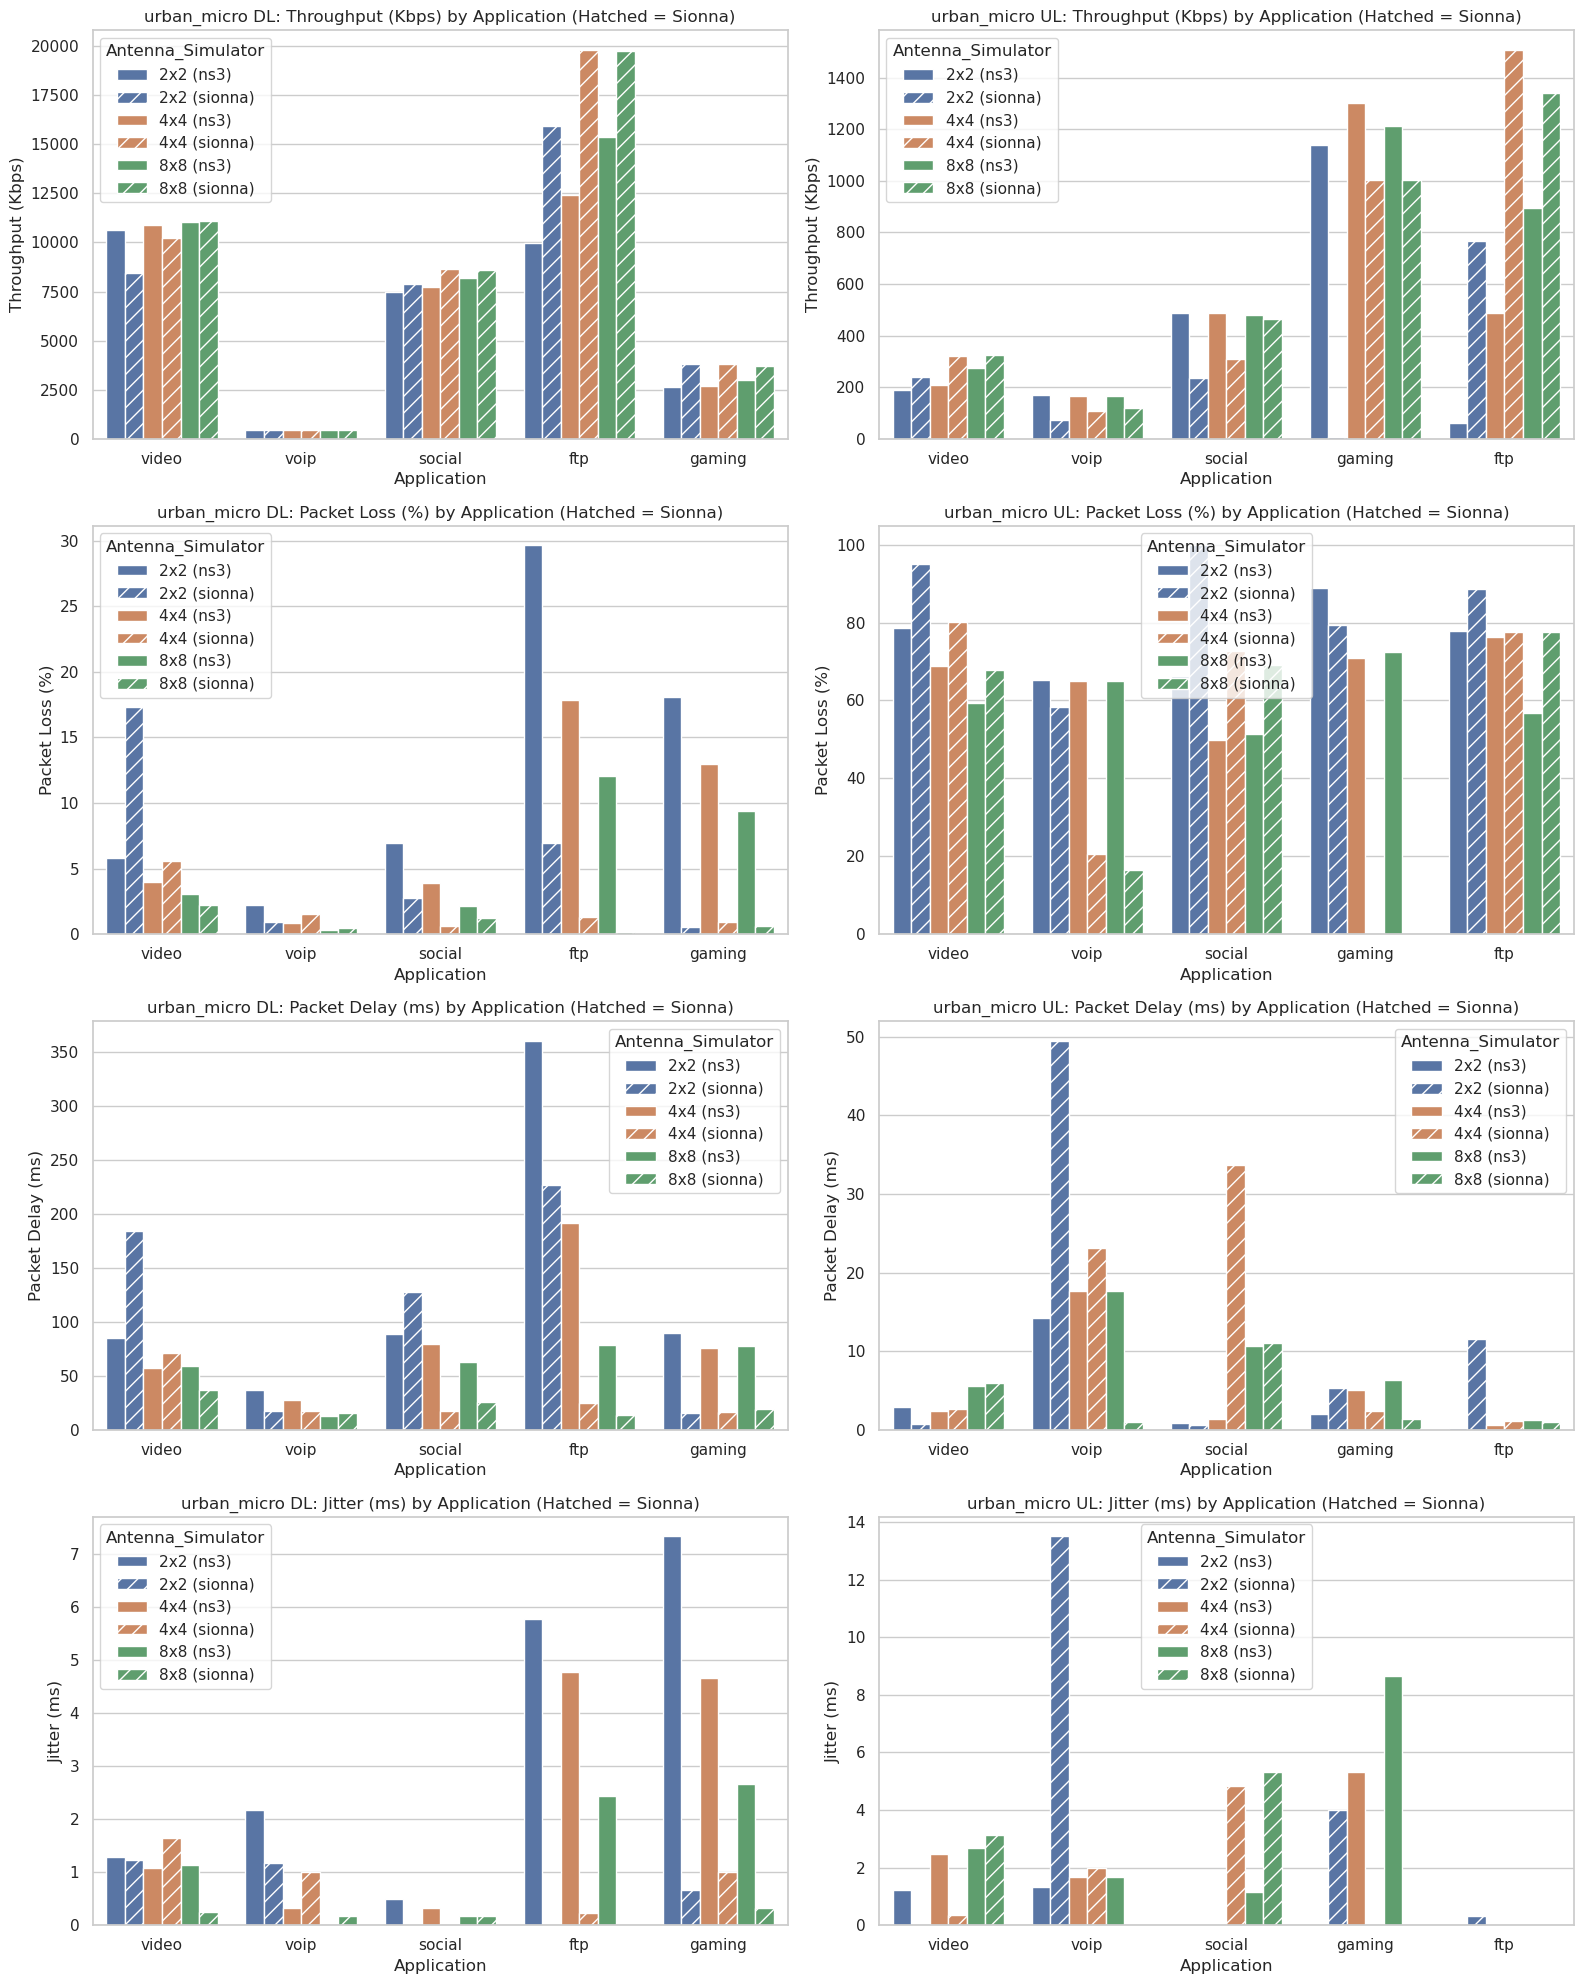
\includegraphics[width=\textwidth]{images/urban_micro_flow_metrics.png}
    \caption{Urban micro Application-related metrics by traffic type, direction, and gNB array size.}
    \label{fig:exp2-urban-micro-flow}
\end{figure*}


\subsubsection{Propagation-related Metrics}
\label{subsubsec:exp2-urban-micro-propagation}

The propagation-related results are presented in Figure \ref{fig:exp2-urban-micro-propagation}.
Average path loss, received power remain consistent across all antenna size at roughly $95.5$ dB and $-62.5$ dBm for both simulators.
Both ns-3 and Sionna RT report nearly identical values for propagation related metrics.

The simulators diverge on path delay and channel quality metrics.
As in the macro scenario (Section~\ref{subsec:exp2-urban-macro}), Sionna~RT reports a higher mean path delay ($178$~ns vs.\ $120$~ns for ns-3), consistent with its multipath-aware propagation accounting over the dense street-level geometry.

Similarly, Sionna RT predicts lower average CQI and MCS values compared to ns-3.
For instance, in the $2 \times 2$ configuration, Sionna RT reports an average CQI of $6$ and MCS of $10$ while ns-3 estimates a CQI of $9.5$ and MCS of $16.5$.
The lower CQI and MCS values in Sionna RT highlight the impact of the detailed multipath fading and interference captured by the ray tracer, leading to a harsher but more realistic channel quality assessment.
Nevertheless, as the antenna array size scales from $2 \times 2$ to $8 \times 8$, both CQI and MCS improve significantly in both simulators.
This further confirms that larger arrays are essential for overcoming the harsh mmWave urban channel.


\begin{figure*}[t]
    \centering
    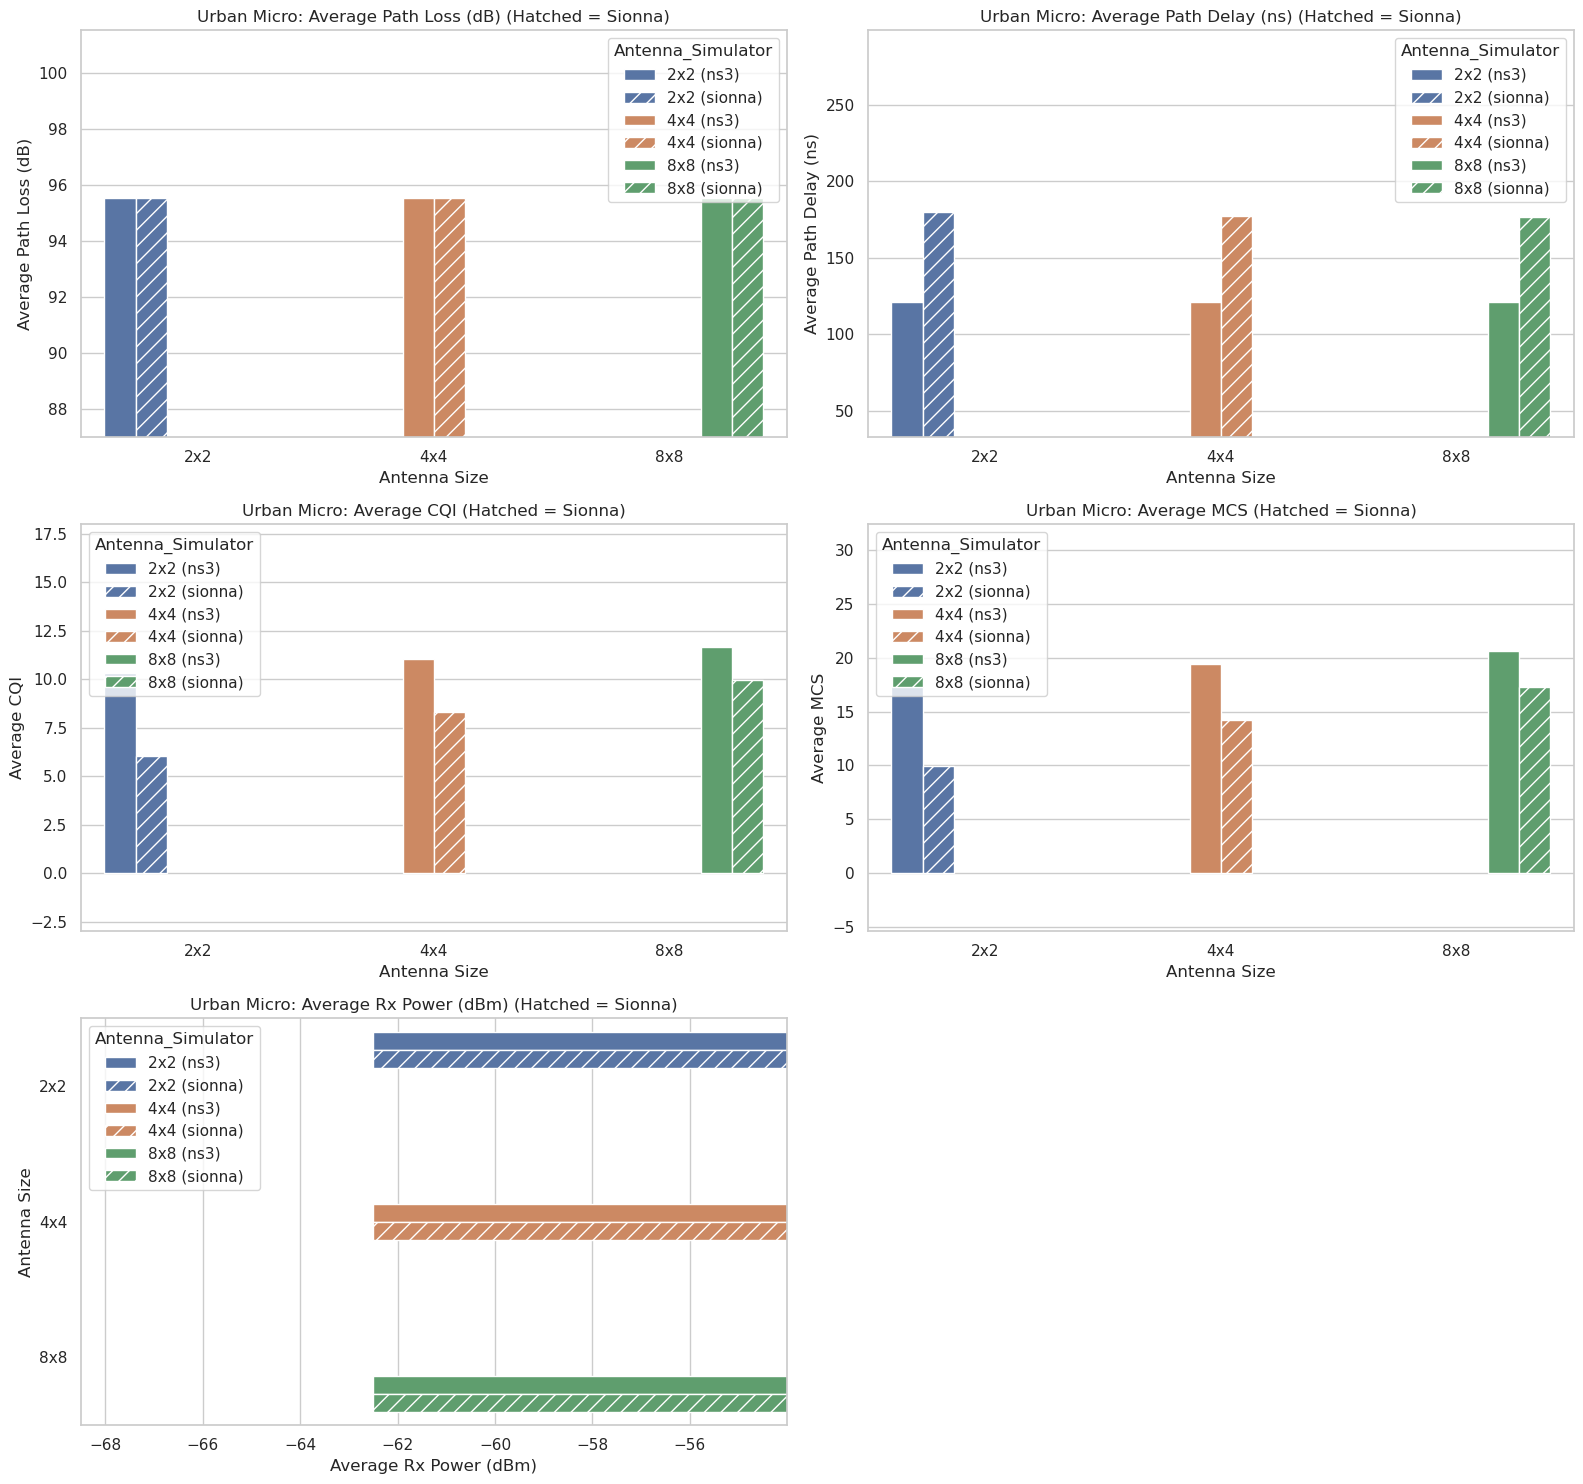
\includegraphics[width=\textwidth]{images/urban_micro_propagation_metrics.png}
    \caption{Urban micro propagation-related metrics by channel mode and gNB array size.}
    \label{fig:exp2-urban-micro-propagation}
\end{figure*}


\subsubsection{Energy Consumption-related Metrics}
\label{subsubsec:exp2-urban-micro-energy}

In Figure \ref{fig:exp2-urban-micro-energy}, the energy consumptions of gNB and UEs by array size, and traffic load are presented.
The gNB energy scaling pattern mirrors the macro scenario: power increases with both array size and traffic load, and Sionna~RT reports slightly lower consumption than ns-3 under high load due to its lower CQI/MCS estimates altering resource allocation.
Under low load, both simulators report $23$~W, $33$~W, and $68$~W for $2\times2$, $4\times4$, and $8\times8$ respectively.
The urban micro scenario adds a notable high-load extreme: the $8\times8$ configuration reaches $215$~W (ns-3) and $193$~W (Sionna~RT) — roughly three times the macro high-load figure — driven by the combined demand of a 400~MHz mmWave channel and dense multipath-induced retransmissions.

UE power consumption ($0.05$~W at low load, $0.09$~W at high load) is nearly identical between the two simulators and independent of gNB array size, confirming that UEs are operating at near-maximum transmit power against the challenging urban channel regardless of the gNB configuration.

\begin{figure*}[t]
    \centering
    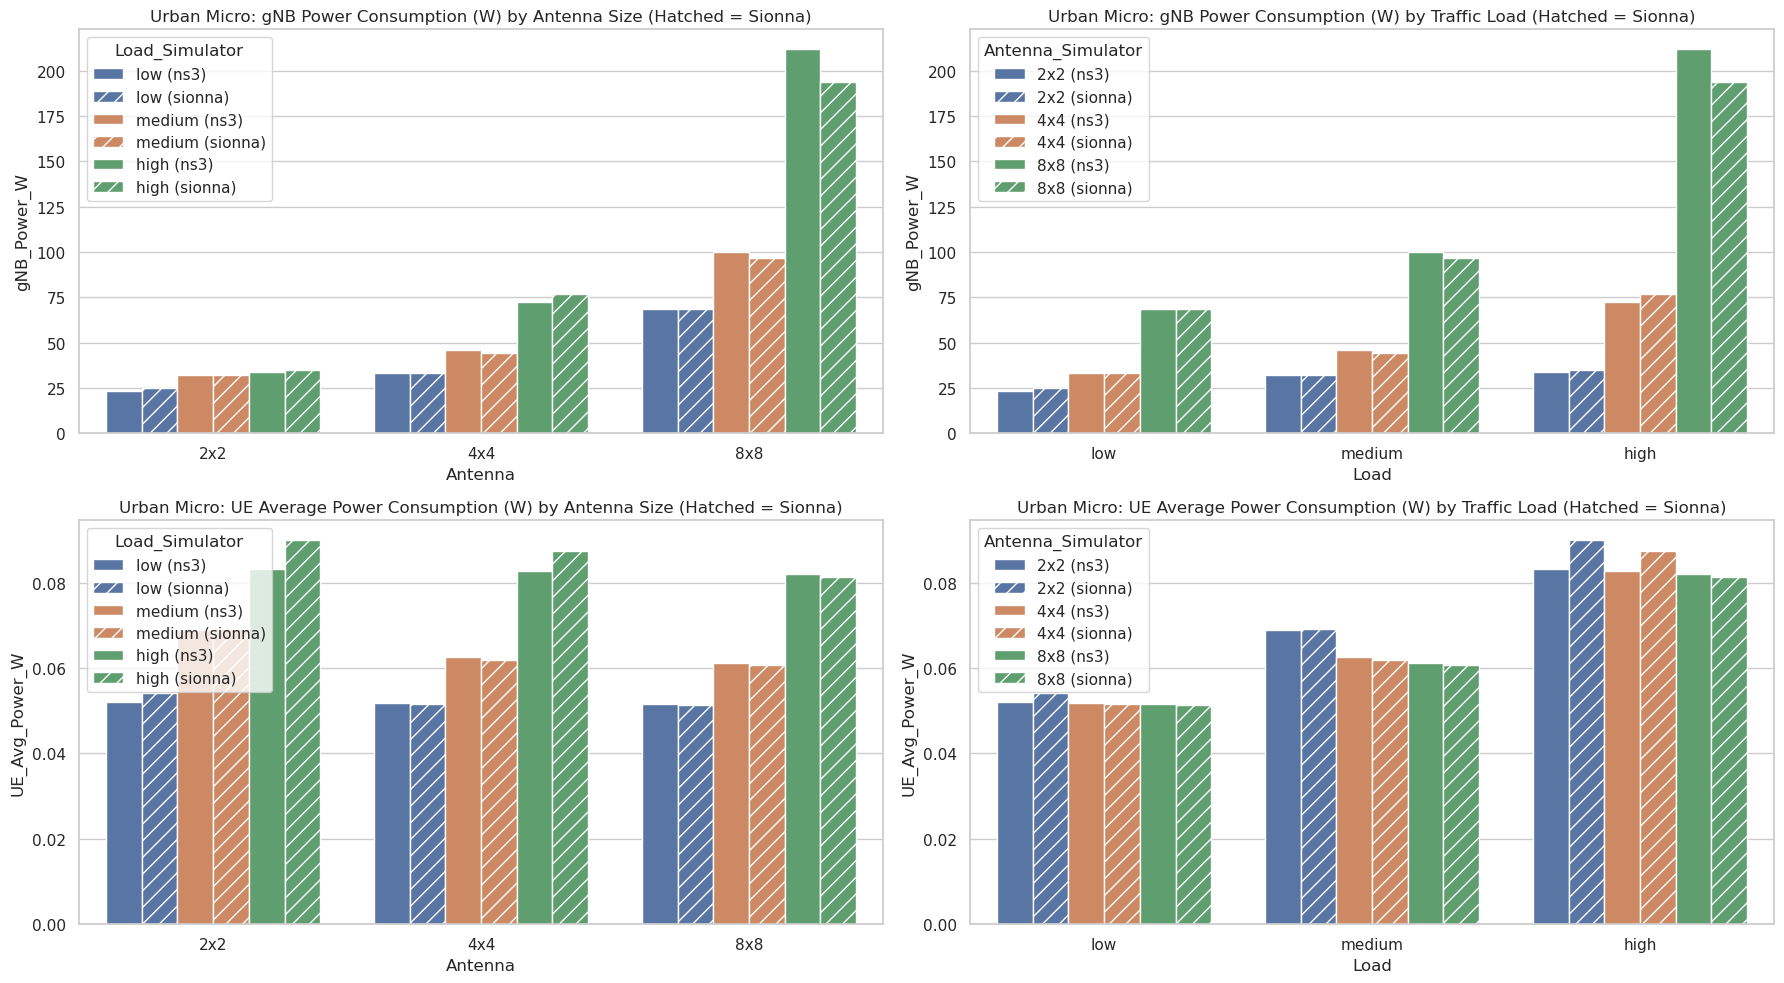
\includegraphics[width=\textwidth]{images/urban_micro_power_consumption.png}
    \caption{Urban micro energy consumptions of gNB and UEs by array size, and traffic load.}
    \label{fig:exp2-urban-micro-energy}
\end{figure*}
